\section{A Re-Imagined Leaderboard Dashboard}
\label{ch:isicle:vis}
\prtodoi{Move to separate demo paper}

Basing a new leaderboard on \irt{} models has another significant benefit: as they are purposefully interpretable, they are very useful for visualizing leaderboard data.
The final component of this work is a demonstration---based on \squad{}---of components that a re-imagined leaderboard may have.\footnote{
    The visualization doubles as my course project for CMSC734: Information Visualization.
}
Our proposed visualization has three main components: (1) an improved model listing, (2) a model-centric view, (3) an example-centric view.

The majority of leaderboards list only one ranking metric or list multiple while only ordering models by a primary metric.
However, multiple factors---including multiple metrics---should be integrated such as model size and efficiency~\citep{strubell2019energy}.
This presents a challenge: how should all these be visualized?
In our proposed model listing, while there would be a default ranking, our visualization would support ranking by any metric or combinations of rankings while showing the influence of each as in the parallel axis plots in LineUp~\citep{gratzl2013lineup}.

\begin{figure}[ht]
    \centering
    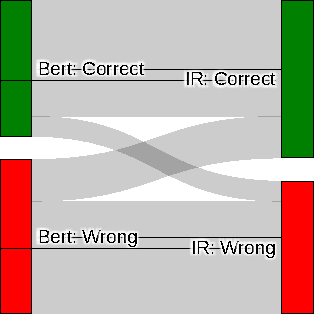
\includegraphics[width=.25\columnwidth]{end_error_compare}
    \caption{
        A proof-of-concept visualization that compares two models---a \bert{} and \ir{} retrieval system---by visualizing which examples model agree or disagree on.
        We propose extending this to incorporate more than two models.
    }
    \label{fig:pair}
\end{figure}

Similarly to Manifold~\citep{zhang2019manifold}, the goal of the model-centric view is to understand the differences---based on predictions---between models.
An initial approach (Figure~\ref{fig:pair}) compares how pairs of models differ, but could be extended to support multiple models by enhancing the underlying software.
Another approach to a model-centric views instead attempts at characterizing the performance along partitions of the data~\citep{liu2018answer}.
For example, \citet{arendt2020crosscheck} propose faceted histograms as a way to ``un-aggregate'' metrics to inspect \qa{} accuracy by factors like question type and confidence.
In addition to visualizing which instances pairs of models agree as in Manifold, we propose integrating \irt{} parameters to better identify instances that have a larger influence over the output ranking.

A dominant approach to inspecting models examines their performance on individual examples or partitions of examples sharing a trait~\citep{wadhwa2018compare}.
In addition to domain-relevant traits, we can guide example sample selection with \irt{} which makes it more likely to identify important issues over random sampling~\citep{wadhwa2018compare} while still combining careful specification of error types~\citep{wu2019errudite}.
Similarly, visualizations can use the multidimensional \irt{} parameters for clustering which can also be combined with domain-specific attributes like question type or topic.

A major advantage of our approach---embedding these comparisons in leaderboards---is that model developers can compare the outputs of many models on individual or small sets of examples.
While there are numerous tools for comparing models, error analysis, and related tasks, they face the headwinds of convincing practitioners that they are worthwhile time investments.
Instead, we aim to provide real benefits of leaderboard-wide analysis without incurring up-front time commitment from practitioners.
Although this does require commitment from task organizers, we believe that the trade-off of inherently improving the evaluation while providing practitioners with ``shiny tools'' is well worth it.
